\documentclass[11pt]{article}
\usepackage[top=1.00in, bottom=1.0in, left=1in, right=1in]{geometry}
\renewcommand{\baselinestretch}{1.1}
\usepackage{graphicx}
\usepackage{natbib}
\usepackage{amsmath}

\begin{document}
\bibliographystyle{/Users/Lizzie/Documents/EndnoteRelated/Bibtex/styles/besjournals}
\renewcommand{\refname}{\CHead{}}

\hspace{-5ex} \includegraphics[width=0.5\textwidth]{/Users/Lizzie/Documents/Professional/images/letterhead/ubc/Faculty of forestry.png}
\pagenumbering{gobble}
\vspace{1.5ex}\\

\setlength{\parindent}{0pt}
\setlength{\parskip}{7pt}
\today

Dear Associate Editor:

Thank you for handling of our manuscript, ``A four-step Bayesian workflow for improving ecological science'' (FEE24-0250), for Concepts and Questions in \emph{Frontiers in Ecology and the Environment}. We were obviously disappointed with the decision to decline our submission and we are writing to ask if you might be willing to consider an appeal. As we detail below, we believe our manuscript offers a novel viewpoint that is very timely, but that may be under-appreciated by statistical experts in the field. We reached out to Dr. Collins to discuss this, and he suggested we contact you directly. 

This is our second review at a high-impact ecology journal and it is becoming apparent that it attracts very split reviews; we believe this reflects the novel niche space our paper tries to fill. In both cases, we had one reviewer being extremely positive, and the other(s) feeling the paper needed to be longer, showcase a more complex statistical example and give generally more detail. One of the main goals of our paper, however, is making the workflow we outline (which is also novel, as we detail below) as approachable as possible to non-statisticians. As Reviewer 2 notes:
\begin{quote}
I commend the authors on condensing a large swath of information into a short, easily digestible piece of work. While a part of me
wanted more (more steps, more examples, more elaboration), I think the real value of this lies in its
brevity and the paired Markdown file.
\end{quote}
We argue that part of the barrier to taking up the approach we outline is that related Bayesian approaches and statistical workflows are often complex and dense, and this has provided a barrier to their uptake in ecology. We chose an example that is simple, but shows the power of the workflow we outline (and the analysis shown was published in \emph{PNAS}, so we do not see it as `overly' simple). Further, we have had the manuscript read by a number of quantitative ecologists who are new to simulating data and/or Bayesian analyses and all have commended how simple and approachable the paper is. 

Bridging the gap that often separates statisticians and applied quantitative ecologists is one part of the novelty of our manuscript, but the other is the specific workflow steps we outline. Combining simple but powerful and organized steps centered around data simulation into a scientific and statistical workflow is considered new according to the broader literature, with \emph{Nature Reviews} publishing a major paper on the novelty and importance of this type of workflow recently \citep[this may be the Gelman publication Reviewer 3 mentions,][though the workflow we outline is distinct from this one co-authored by Gelman]{vandeschoot2021}, that has been recently followed by extensions to other fields \citep[for example in epidimeology, veterinary and cognitive sciences,][]{grinsztajn2021,schad2021,mielke2023workflow,hess2024bayesian} but it is not well integrated into ecology. Indeed, \emph{Philosophical Transactions of the Royal Society A} has just commissioned a special issue on the value of the type of workflow we outline (one of us, EMW, has been invited a co-editor on this special issue) across different fields. 

We thus believe the reviewers' comments that this is not novel are misleading. There is not an equivalent paper by Gabry, he has published only very specifically on visualization within workflows. Further, the two papers cited by Reviewer 1 are specific to data assimilation for ecological forecasting, not data simulation for improving ecological approaches across the sub-disciplines of the field. While we understand some statistical experts may feel that they follow these steps already, the wider ecological community does not. The field lacks a clear paper on appropriate methods to follow for these steps, and on the process of combining them into a useful workflow. 

After reviewing comments from reviewers we feel that we could address most of them straightforwardly; some require simple clarifications, while others highlight areas of misunderstanding, in part reflecting the divide our manuscript attempts to bridge. We realize, however, that we may never convince some statistical experts of the novelty of our paper, they will continue to find it too simple and believe it outlines what they already do (which may be true for some of them). But this is not the readership our paper addresses. Our paper is targeted at the large number of ecologists adopting complex, often Bayesian, statistical analyses and looking for guidance in how to make their analyses more robust and reproducible---and we believe \emph{Frontiers in Ecology and the Environment} is the place to help break through on this new workflow. We think even some of the reviewers see this tension (e.g., Reviewer 1 who was `fairly torn') and may be convinced by a revision addressing their concerns. 

We hope you will consider our request for a chance to revise this manuscript and would be happy to answer any questions or provide additional responses to reviewer concerns. 

\iffalse
The manuscript is authored by an international and interdisciplinary group of ecologists, conservation biologists and statisticians. The workflow follows the basics of how authors EM Wolkovich, TJ Davies and WD Pearse approach model building and leverages the insights and skills of computational statistician M Betancourt who has developed fundamental statistical workflows for diverse scientific disciplines. We have designed it to be broadly generalizable and practical, including relevant examples of forecasting shifts in animals and plants over time.

% We hope that you will find this perspective, which provides a road-map for the many different practitioners in ecology now building more complex models, suitable for publication in \emph{Frontiers in Ecology and the Environment}. % By integrating simulation more fully in model building and testing this workflow can fit models that are more robust and well-suited to provide new ecological insights---allowing us to refine where to put resources for better estimates, better models, and better forecasts. 
All authors contributed to this work, which is our original work and not pre-published, and we declare no conflict of interest (following ESA's Code of Ethics). The manuscript is 2690 words plus 140 word summary and a 100-word in a nutshell; it has three figures and one glossary. It is not under consideration elsewhere.  % This manuscript is not under consideration elsewhere, and all authors approved of this version for submission. 
\fi

Sincerely,\\

\includegraphics[scale=1]{/Users/Lizzie/Documents/Professional/Vitas/Signatures/SignatureLizzieSm.png} \\

Elizabeth M Wolkovich\\
Associate Professor of Forest \& Conservation Sciences\\ 
University of British Columbia\\

\newpage
{\bf References}
\vspace{-8ex}
\bibliography{..//refs/bayesrefsmini.bib}



\end{document}

\newpage
{\bf Example figures}


\begin{figure}[ht]
\centering
\noindent 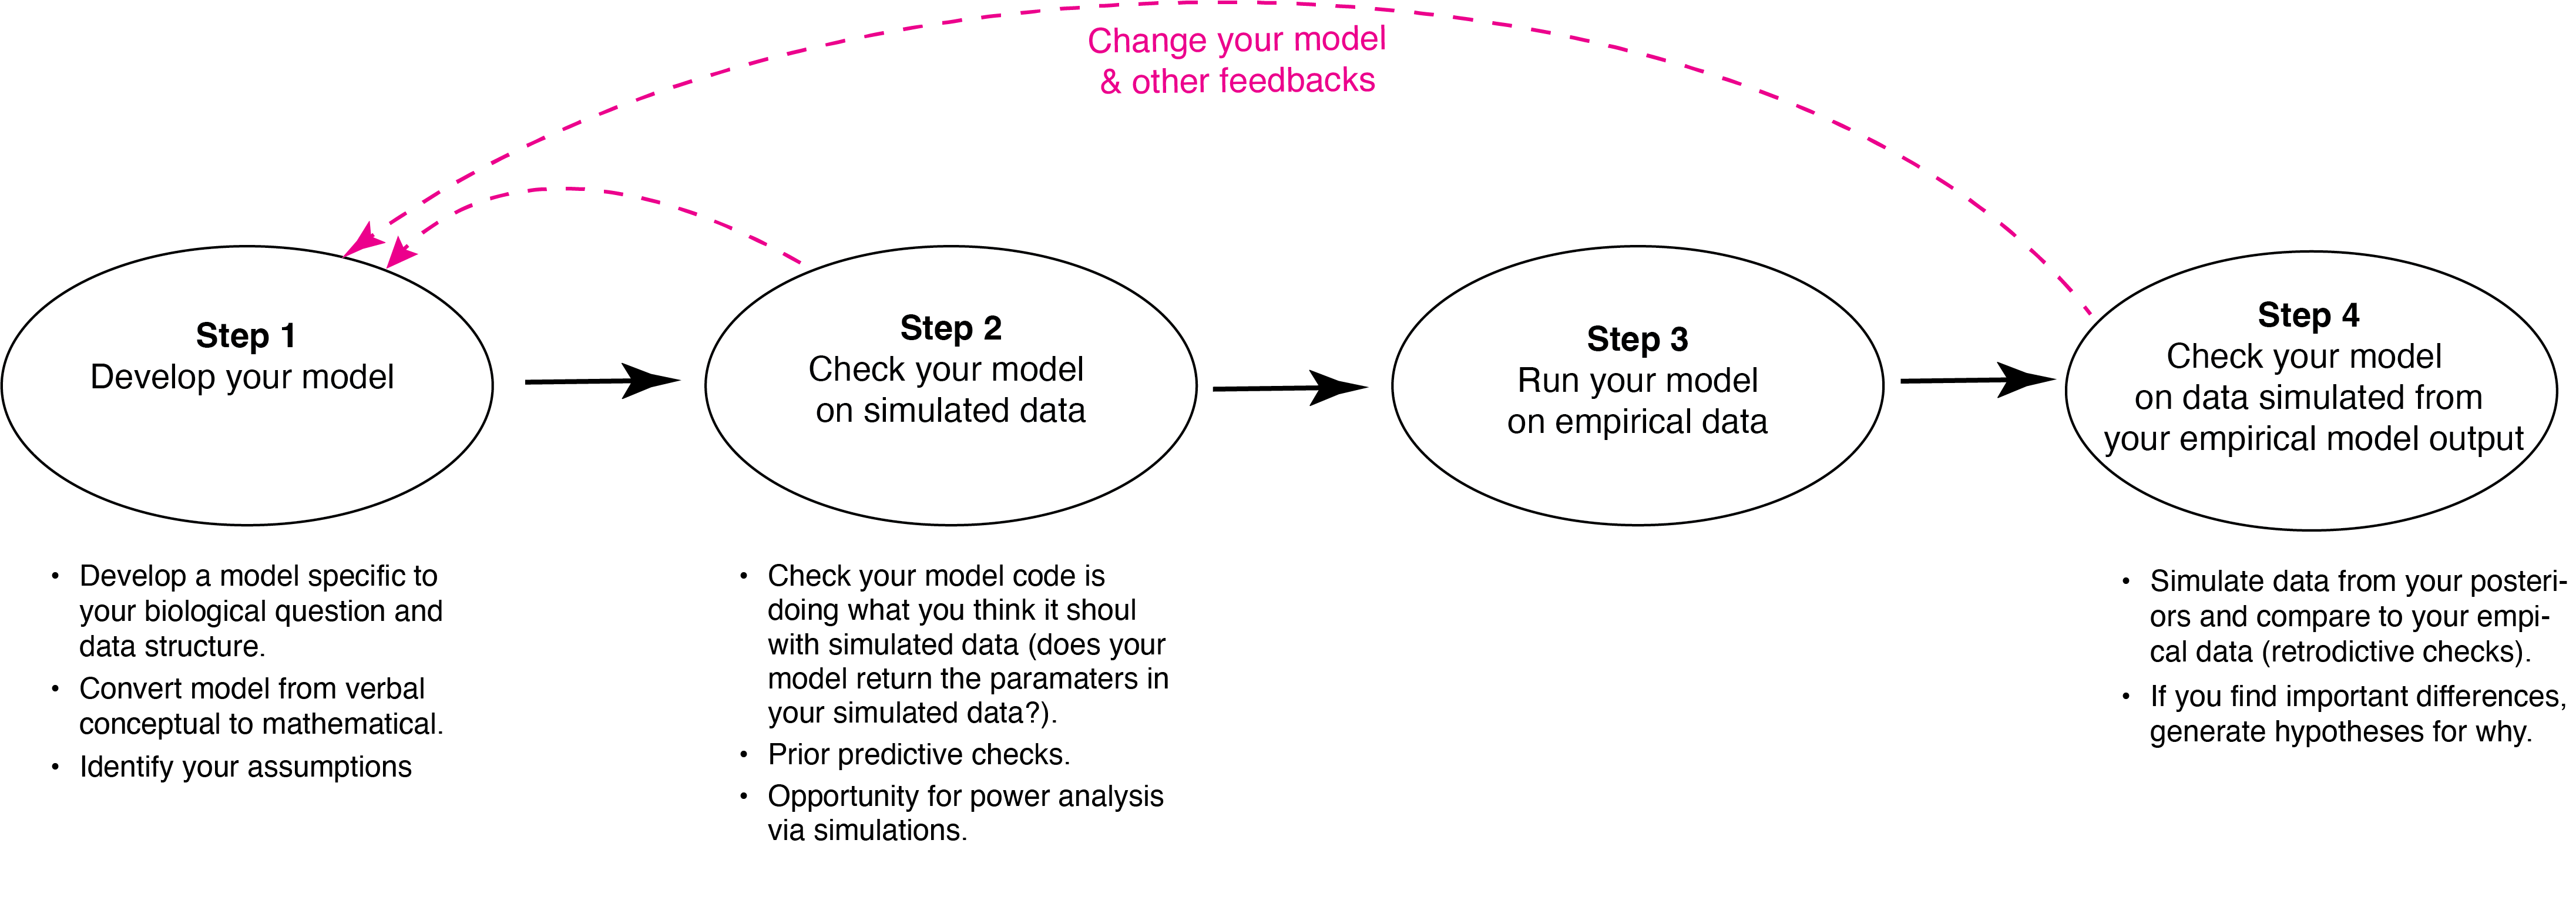
\includegraphics[width=1\textwidth]{..//figures/workflow.png}
\caption{The four-step iterative workflow we outline can help design models for specific ecological questions, data and aims---which makes this a statistical workflow that can naturally become a scientific workflow. It makes the step that many of us focus on---running your model on your empirical data (Step 3)---far more straightforward and insightful by using simulations both before (Step 2) and after (Step 4) it to better understand the model and data together.}
\label{fig:workflow}
\end{figure}

\begin{figure}[ht]
\centering
\noindent 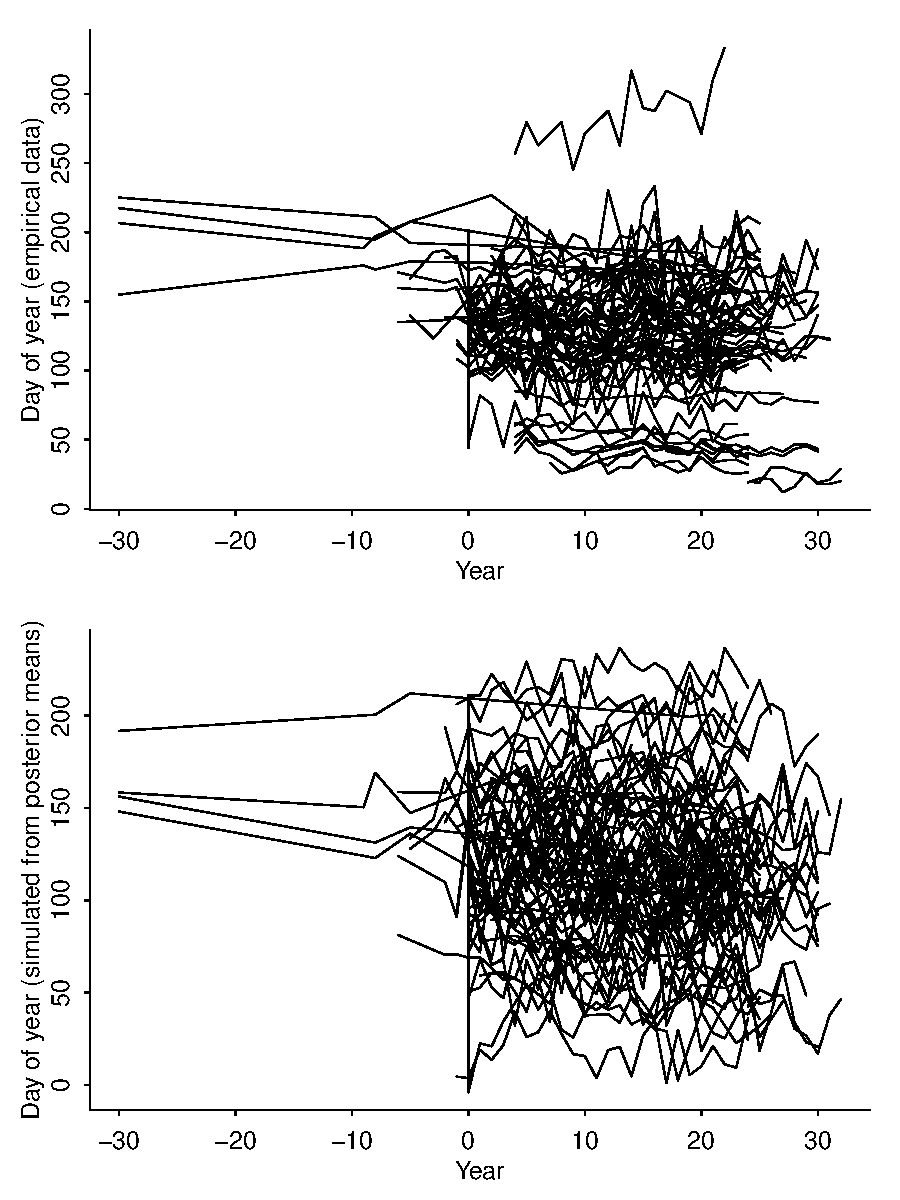
\includegraphics[width=0.6\textwidth]{..//examples/synchrony/graphs/rawvsonepredictivecheck.pdf}
\caption{Example of a single retrodictive check from time-series data of phenological events over time. The raw data (top, black) looks similar to one simulated dataset (bottom, purple), based on existing species number, their respective $x$ data, and simulating from the parameters for each species. See `An example workflow' in the Supplement for more details.}
\label{fig:retrodictivecheck}
\end{figure}


%%%
%%%

\begin{figure}[ht]
\centering
\noindent 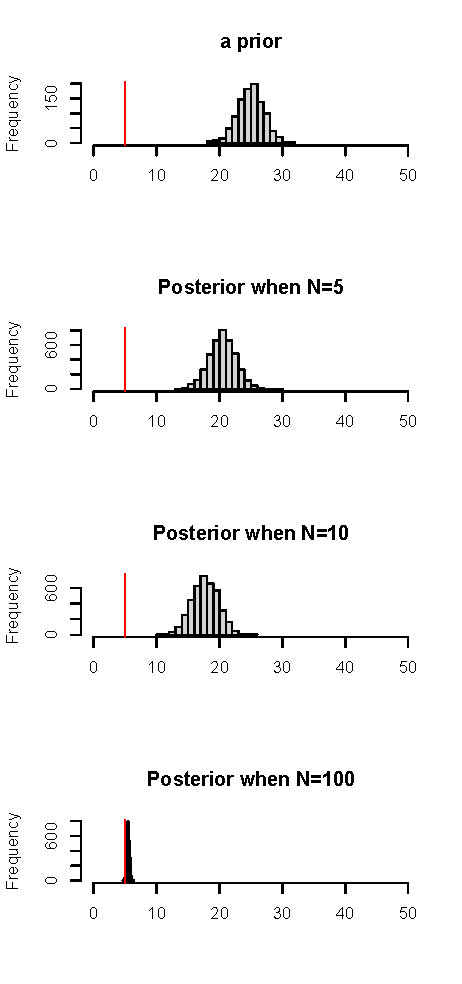
\includegraphics[width=0.5\textwidth]{..//examples/misspecifiedmodel/priorpostforflows.pdf}
\caption{A simple example of how to use simulated data to understand calibration issues in a mis-specified model. Here we know the true model underlying the data is $y=\alpha + \text{normal}(0, \sigma)$ where $\alpha$ is 5 (shown as blue vertical line) and $\sigma$ is 2. The model, however, is mis-specified by a prior for $\alpha$ of $\text{normal}(25, 2)$ (dashed blue line), resulting in a posterior (salmon-colored histogram) not centered on the true value. In our experience it is quite rare to have a prior informed by ecological knowledge be so far off, but this is an example. How mis-calibrated the model will be depends on the data: we show examples with a sample size ($N$) of 5, 10 and 40 data points. In practice these studies would allow us to determine how much data we would need to be robust to suspect prior models. (Note the change in $y$ axis range for bottom plot.) }
\label{fig:misspecifyprior}
\end{figure}


